% =====================================================================
%  Chapter 3 -- Experimental set-up and methods
% =====================================================================
\chapter{Experimental Set-up and Methods}\label{ch:methods}
\chapterlists


% ---------------------------------------------------------------------
\section{The circuit}\label{sec:circuit}

The oscillator of \cref{fig:wien-basic} is built on a breadboard around an LM741 operational amplifier
with a $\pm\SI{15}{\volt}$ supply (\cref{fig:photos}), with $R=\SI{2.17}{\kilo\ohm}$ and
$C=\SI{1}{\micro\farad}$ ($f_{0}\approx\SI{73}{\hertz}$, \cref{eq:omega0-value}). Its output
saturates at $\Asat\approx\SI{11.2}{\volt}$. The gain is controlled by a \SI{10}{\kilo\ohm}
digital potentiometer with 32 wiper positions, set by a microcontroller and placed in series with a fixed
resistor in one of two configurations (\cref{fig:two-configs,tab:configs}).

\begin{figure}[!htb]
\centering
\begin{subfigure}[b]{0.49\linewidth}
\centering
\begin{circuitikz}[font=\footnotesize,scale=0.8,transform shape]
  \ctikzset{bipoles/length=0.85cm}
  \draw (0,0) node[op amp, noinv input up] (oa) {};
  \draw (oa.out) -- ++(1.6,0) coordinate (O) node[right] {$\Vout$};
  \coordinate (N) at ($(oa.-)+(-0.5,0)$);
  \draw (oa.-) -- (N) -- ++(0,-1.3) coordinate (B);
  \draw (B) to[R, l_=\SI{91}{\kilo\ohm}, *-] ++(1.9,0) coordinate (M) to[vR, color=accent] (B -| O) -- (O);
  \draw (B) to[R, l_=\SI{47}{\kilo\ohm}] ++(0,-1.7) node[ground]{};
  \coordinate (P) at ($(oa.+)+(-1.9,0)$);
  \draw (oa.+) -- (P);
  \draw (P) -- ++(0,1.35) coordinate (T);
  \draw (T) to[R, l=$R$] ++(2.2,0) to[C, l=$C$] (T -| O) -- (O);
  \draw (P) to[C, l=$C$, *-] ++(0,-1.9) node[ground]{};
  \draw (P) -- ++(-0.95,0) to[R, l_=$R$] ++(0,-1.9) node[ground]{};
  \node[draw=accent, rounded corners=2pt, font=\scriptsize, inner sep=3pt] (ard) at ($(M)!0.5!(B -| O)+(0,-1.6)$) {Arduino};
  \draw[-{Stealth[length=1.6mm]}, dashed, color=accent] (ard.north) -- ++(0,0.98);
  \node[font=\scriptsize, color=accent] at ($(B)!0.5!(B -| O)+(0,0.55)$) {$\RF$ (swept)};
\end{circuitikz}
\caption{Configuration A: $\RF$ swept}
\end{subfigure}\hfill
\begin{subfigure}[b]{0.49\linewidth}
\centering
\begin{circuitikz}[font=\footnotesize,scale=0.86,transform shape]
  \ctikzset{bipoles/length=0.9cm}
  \draw (0,0) node[op amp, noinv input up] (oa) {};
  \draw (oa.out) -- ++(1.3,0) coordinate (O) node[right] {$\Vout$};
  \coordinate (N) at ($(oa.-)+(-0.5,0)$);
  \draw (oa.-) -- (N) -- ++(0,-1.25) coordinate (B);
  \draw (B) to[R, l=\SI{90}{\kilo\ohm}, *-] (B -| O) -- (O);
  \draw (B) to[R, l_=\SI{41}{\kilo\ohm}] ++(0,-1.45) coordinate (Q) to[vR, l_=\SIrange{0}{10}{\kilo\ohm}, color=accent] ++(0,-1.45) node[ground]{};
  \coordinate (P) at ($(oa.+)+(-1.9,0)$);
  \draw (oa.+) -- (P);
  \draw (P) -- ++(0,1.35) coordinate (T);
  \draw (T) to[R, l=$R$] ++(2.0,0) to[C, l=$C$] (T -| O) -- (O);
  \draw (P) to[C, l=$C$, *-] ++(0,-1.9) node[ground]{};
  \draw (P) -- ++(-0.95,0) to[R, l_=$R$] ++(0,-1.9) node[ground]{};
  \node[draw=accent, rounded corners=2pt, font=\scriptsize, inner sep=3pt, align=center] (ard) at ($(Q)+(1.75,-0.72)$) {Arduino};
  \draw[-{Stealth[length=1.6mm]}, dashed, color=accent] (ard.west) -- ++(-1.05,0);
  \node[font=\scriptsize] at ($(B)!0.5!(B -| O)+(0,0.75)$) {$\RF$};
  \node[font=\scriptsize, color=accent, anchor=west] at ($(Q)+(0.35,0.75)$) {$\Ri$ (swept)};
\end{circuitikz}
\caption{Configuration B: $\Ri$ swept}
\end{subfigure}
\caption[The two configurations of the experiment]{The two configurations of the experiment. The
digital potentiometer (shown in colour) is driven by an Arduino. (a)~In Stages~1 to~3 it is in series
with a fixed \SI{91}{\kilo\ohm} resistor and forms the feedback resistor $\RF$. (b)~In Stage~4 it is in
series with a fixed \SI{41}{\kilo\ohm} resistor and forms the input resistor $\Ri$. In both cases
$R=\SI{2.17}{\kilo\ohm}$ and $C=\SI{1}{\micro\farad}$.}
\label{fig:two-configs}
\end{figure}

\begin{table}[!htb]
  \centering
  \small
  \renewcommand{\arraystretch}{1.2}
  \begin{tabular}{@{}lcc@{}}
    \toprule
    & \textbf{Configuration A} & \textbf{Configuration B} \\
    \midrule
    Swept resistor & $\RF = \SI{91}{\kilo\ohm}$ + potentiometer & $\Ri = \SI{41}{\kilo\ohm}$ + potentiometer \\
    Range of the swept resistor & \SIrange{91}{101}{\kilo\ohm} & \SIrange{41}{51}{\kilo\ohm} \\
    Fixed resistor & $\Ri=\SI{47}{\kilo\ohm}$ & $\RF=\SI{90}{\kilo\ohm}$ \\
    Range of gain $G$ & 2.94 to 3.15 & 3.20 to 2.76 \\
    Ideal threshold ($\Gc=3$) at & $\RF=\SI{94}{\kilo\ohm}$ & $\Ri=\SI{45}{\kilo\ohm}$ \\
    Change of $G$ per step & 0.0069 & 0.011 to 0.017 \\
    State at the start of a run & quiet & oscillating \\
    Used in & Stages 1 to 3 & Stage 4 \\
    \bottomrule
  \end{tabular}
  \caption[The two circuit configurations]{The two circuit configurations. In B each step changes the
  gain about twice as much as in A.}
  \label{tab:configs}
\end{table}

\begin{figure}[!htb]
  \centering
  \begin{subfigure}[b]{0.49\linewidth}
    \centering
    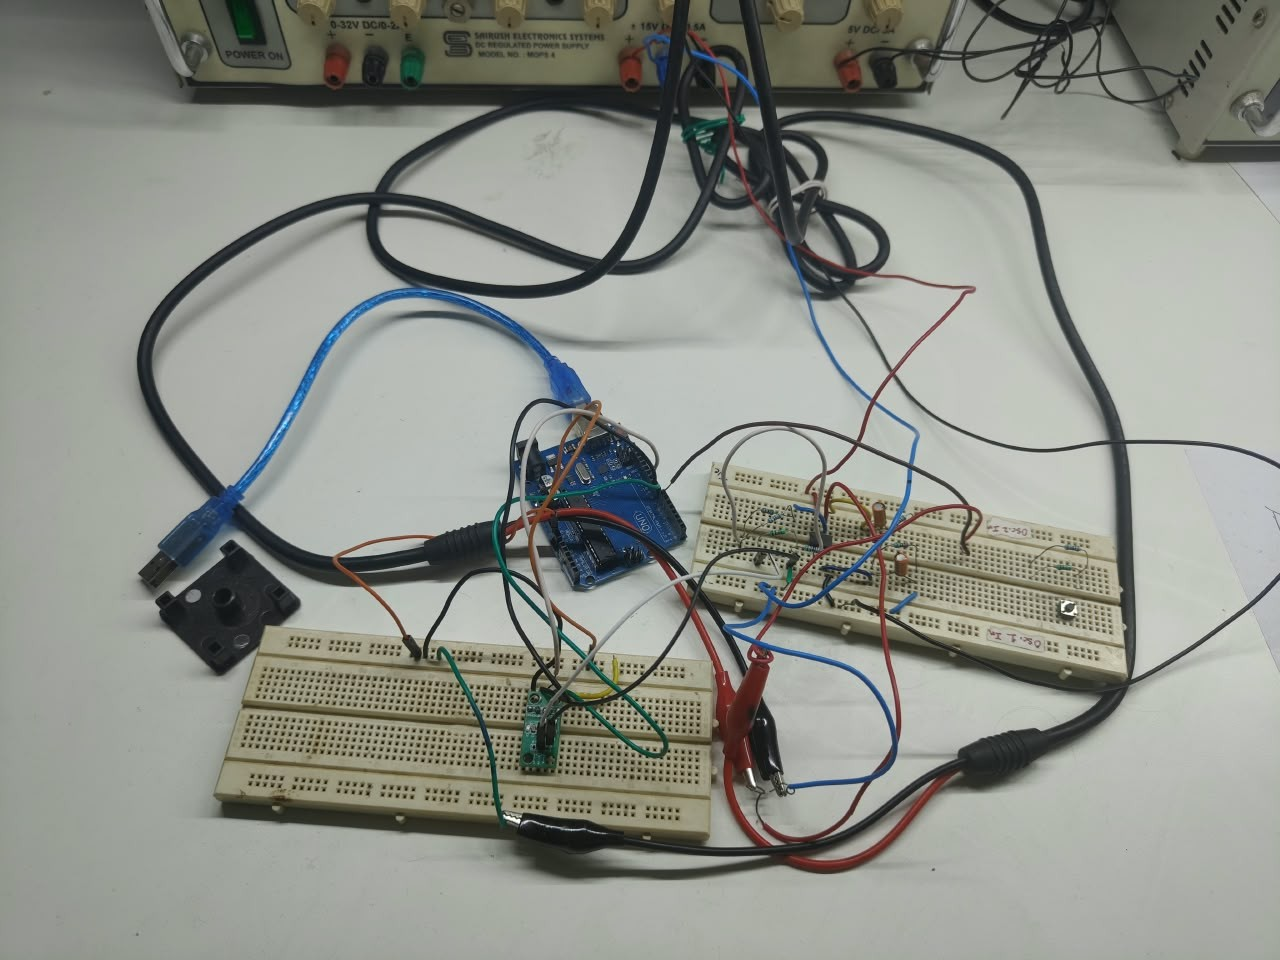
\includegraphics[width=0.85\linewidth]{photo_circuit}
    \caption{The circuit}
  \end{subfigure}\hfill
  \begin{subfigure}[b]{0.49\linewidth}
    \centering
    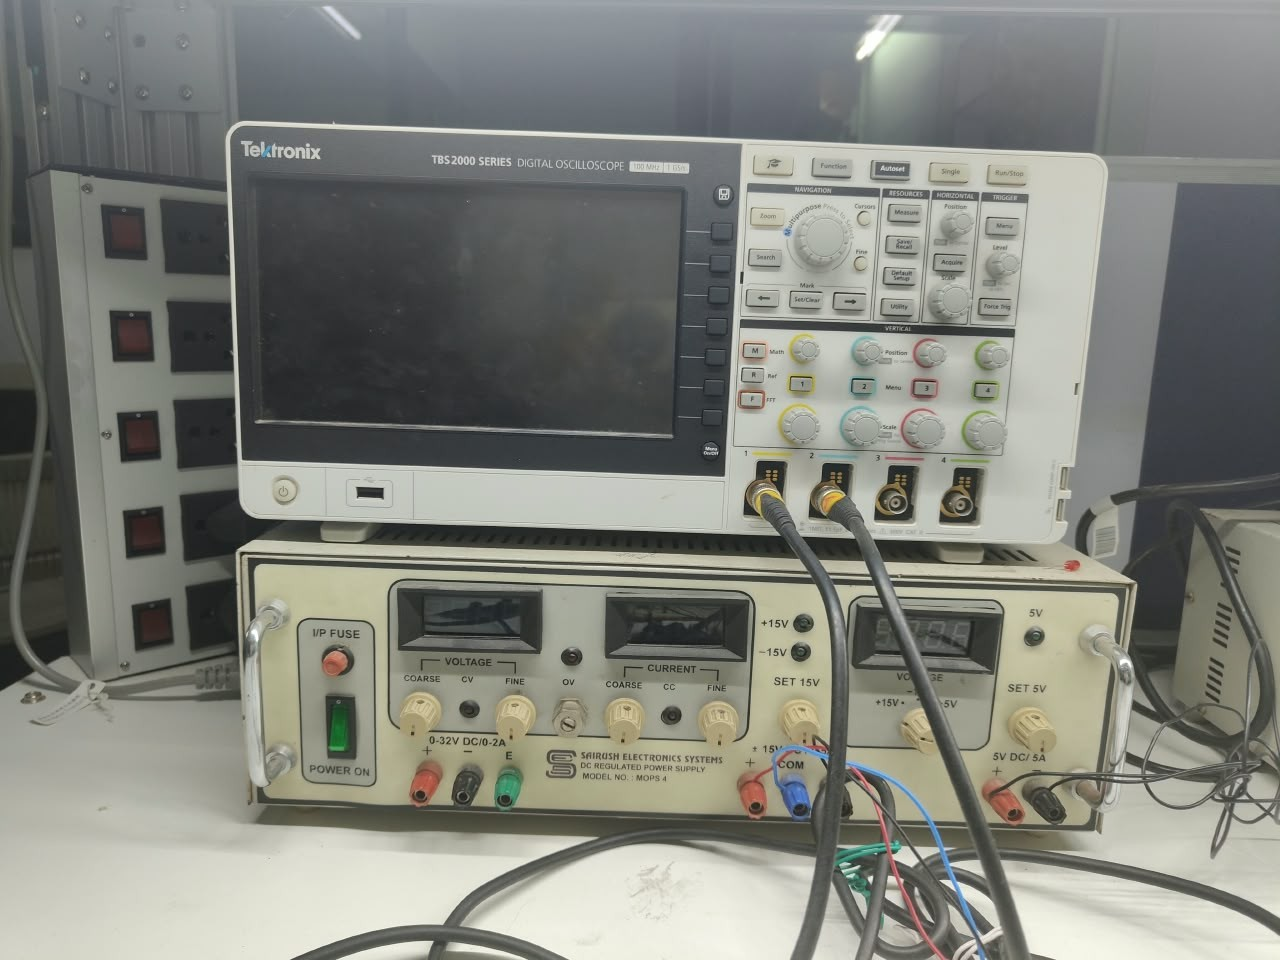
\includegraphics[width=0.85\linewidth]{photo_instruments}
    \caption{Oscilloscope and power supply}
  \end{subfigure}
  \caption[Photographs of the experimental set-up]{The set-up. (a)~Oscillator, digital potentiometer
  and Arduino on breadboards. (b)~Oscilloscope and regulated supply.}
  \label{fig:photos}
\end{figure}

% ---------------------------------------------------------------------
\section{Sweeping the gain: the staircase protocol}\label{sec:protocol}

An Arduino moves the wiper one position at a time, waiting a time $\tau$ after each move: 31 steps
to one end, 31 back, repeated indefinitely. The swept resistance follows a triangular staircase
(\cref{fig:staircase}) with step
\begin{equation}
  \Delta R = \frac{\SI{10}{\kilo\ohm}}{31} = \SI{322.6}{\ohm}
  \label{eq:step}
\end{equation}
and rate $\lambda=\Delta R/\tau$ (\cref{eq:lambda-stair}). The end positions are held for two step
times, so a cycle lasts $64\,\tau$ and every position is occupied for $2\tau$ per cycle, as assumed in
\cref{sec:budget}.

\begin{figure}[!htb]
\centering
\begin{tikzpicture}[x=0.1cm,y=0.085cm]
  % axes
  \draw[-{Stealth[length=2mm]}] (0,0) -- (132,0) node[below left=1pt, font=\footnotesize] {time};
  \draw[-{Stealth[length=2mm]}] (0,0) -- (0,40) node[above right, font=\footnotesize] {swept resistance};
  % staircase: 2 cycles of 64 steps, 32 levels (drawn with level height 1)
  \draw[line width=0.6pt, color=ink]
    (0,2)
    \foreach \c in {0,1} {
      \foreach \k in {0,...,30} { -- ++(1,0) -- ++(0,1) }
      -- ++(2,0)
      \foreach \k in {0,...,30} { -- ++(0,-1) -- ++(1,0) }
      -- ++(1,0)
    };
  \draw[dashed, color=accent, line width=0.5pt] (0,14) -- (130,14) node[above left, font=\footnotesize, color=accent] {$R_{c}$};
  \draw[<->, line width=0.4pt] (0,-4) -- (64,-4) node[midway, below, font=\footnotesize] {one cycle $=64\,\tau$};
  \draw[<->, line width=0.4pt] (-3,2) -- (-3,33) node[midway, left, font=\footnotesize, align=right] {31 steps\\of $\Delta R$};
  % zoom on two steps
  \begin{scope}[shift={(50,40)}]
    \draw[line width=0.3pt, color=soft, rounded corners=1pt] (-3,-3) rectangle (27,17);
    \draw[line width=0.8pt, color=ink] (0,0) -- ++(8,0) -- ++(0,5) -- ++(8,0) -- ++(0,5) -- ++(8,0);
    \draw[<->, line width=0.4pt] (8,3) -- (16,3) node[midway, below, font=\scriptsize] {$\tau$};
    \draw[<->, line width=0.4pt] (18,5) -- (18,10) node[midway, right, font=\scriptsize] {$\Delta R$};
    \node[font=\scriptsize, color=soft, anchor=south west] at (-3,17) {zoom: two steps};
  \end{scope}
\end{tikzpicture}
\caption[The staircase sweep protocol]{The staircase sweep: 31 steps of $\Delta R$ up and down, each
held for $\tau$. The path is identical in every run; only $\tau$, and hence $\lambda=\Delta R/\tau$,
changes.}
\label{fig:staircase}
\end{figure}

\textbf{The path is the same in every run}: the same 32 values in the same order. Only $\tau$ changes,
so any difference between runs is due to the rate alone, as Criterion~3 requires. At the start of each
run the Arduino sends a trigger pulse to a second oscilloscope channel, fixing the origin of time and
hence the wiper position at every instant.

\paragraph{Nominal and true rates} To keep the microcontroller arithmetic simple, the step time was
programmed as $\tau = \SI{312.5}{\ohm}/\lambda$, dividing the \SI{10}{\kilo\ohm} span by the 32
positions instead of the 31 intervals. The true step is \SI{322.6}{\ohm} (\cref{eq:step}), so true
rates exceed nominal ones by $3.2\%$, a systematic error of about $3\%$. Runs are \emph{labelled} by
nominal rate or step time; every rate in a plot or fit is the true rate, from the true step and the step
time measured in the recording.

% ---------------------------------------------------------------------
\section{Recording the output}\label{sec:acquisition}

Output and trigger are recorded on a Tektronix TBS2000-series oscilloscope, with a sampling interval
(\SIrange{0.08}{8}{\milli\second}) chosen per run to hold several cycles while resolving the
oscillation. In configuration A, 17 rates (\SIrange{100}{9000}{\ohmpersec}) were recorded with five
cycles each; in configuration B, 19 runs with $\tau=\SIrange{37}{100}{\milli\second}$, each at least
\SI{60}{\second} long (12 to 28 cycles). \Cref{fig:procedure} summarises the procedure.

\begin{figure}[!htb]
\centering
\begin{tikzpicture}[node distance=0.33cm,
    box/.style={draw=accent, line width=0.5pt, rounded corners=2pt, fill=boxbg, font=\footnotesize,
                text width=5.4cm, align=center, inner sep=4pt, minimum height=0.62cm},
    arr/.style={-{Stealth[length=1.8mm]}, line width=0.5pt, color=soft}]
  \node[box] (a) {Choose the step time $\tau$ (sets the rate $\lambda$)};
  \node[box, below=of a] (b) {Arduino starts the sweep and sends the trigger pulse};
  \node[box, below=of b] (c) {Potentiometer steps up and down along the fixed path};
  \node[box, below=of c] (d) {Oscilloscope records $\Vout$ and the trigger};
  \node[box, below=of d] (e) {Record stored after several complete cycles};
  \node[box, below=of e, fill=keybg, draw=ink] (f) {Repeat with a new step time};
  \foreach \x/\y in {a/b,b/c,c/d,d/e,e/f} \draw[arr] (\x) -- (\y);
  \draw[arr] (f.west) -- ++(-0.9,0) |- (a.west);
\end{tikzpicture}
\caption[Procedure for one run]{The procedure for one run of the experiment.}
\label{fig:procedure}
\end{figure}

% ---------------------------------------------------------------------
\section{Challenges and rectifications}\label{sec:challenges}

\begin{itemize}
  \item \textbf{Step count and range.} The first sweep assumed a 100-position potentiometer and the wrong
        gain range, so the threshold was crossed at an unknown, uneven rate. Redesigning around the real
        32 positions and a range straddling the threshold gave configuration A.
  \item \textbf{Time reference.} Without a start marker the resistance at a given instant was unknown;
        the trigger pulse fixed this.
\end{itemize}

% ---------------------------------------------------------------------
\section{From a recording to numbers}\label{sec:analysis}

Each recording is reduced to a few numbers (\cref{fig:pipeline,fig:reading}):

\begin{figure}[!htb]
\centering
\begin{tikzpicture}[node distance=0.32cm,
    box/.style={draw=accent, line width=0.5pt, rounded corners=2pt, fill=boxbg, font=\footnotesize,
                text width=2.2cm, align=center, inner sep=3pt, minimum height=1.35cm},
    arr/.style={-{Stealth[length=1.8mm]}, line width=0.5pt, color=soft}]
  \node[box] (a) {\textbf{Envelope}\\ amplitude of $\Vout$ against time};
  \node[box, right=of a] (b) {\textbf{Events}\\ 90\% on the rise, 10\% on the decay};
  \node[box, right=of b] (c) {\textbf{Position}\\ time of each event $\rightarrow$ resistance};
  \node[box, right=of c] (d) {\textbf{Average}\\ over the cycles of the run};
  \node[box, right=of d, fill=keybg, draw=ink] (e) {\textbf{Fit}\\ against the sweep rate};
  \foreach \x/\y in {a/b,b/c,c/d,d/e} \draw[arr] (\x) -- (\y);
\end{tikzpicture}
\caption[The analysis of a recording]{The analysis applied to every recording, experimental or
simulated.}
\label{fig:pipeline}
\end{figure}

\begin{figure}[!htb]
  \centering
  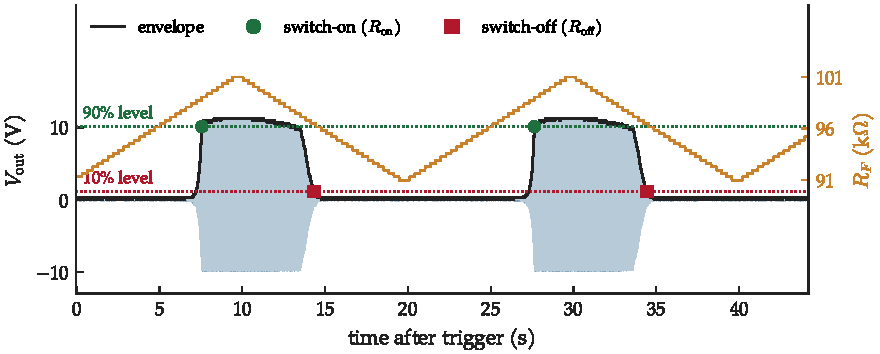
\includegraphics[width=0.7\linewidth]{fig_s2_reading}
  \caption[Reading a recording]{Reading a recording (configuration A, \SI{1}{\kilo\ohm\per\second}
  nominal). Switch-on: envelope (black) rising through 90\%; switch-off: falling through 10\%. The
  staircase (orange) gives the resistance at each instant.}
  \label{fig:reading}
\end{figure}

\begin{enumerate}[label=\arabic*.]
  \item \textbf{Envelope:} running maximum of the output over about two periods.
  \item \textbf{Events:} in each cycle, switch-on where the envelope rises through $90\%$ of $\Asat$ and
        switch-off where it falls through $10\%$, the levels of \cref{eq:Lon,eq:Loff}.
  \item \textbf{Resistance:} using the trigger and the measured step time, each event time is converted
        into the swept resistance, giving $\Ron$ and $\Roff$ per cycle. The staircase is replaced by the
        straight line through the middle of every step; for a gain linear in the resistance this line
        accumulates exactly the same growth, $\int\sigma\,\dd t$, as the staircase, so the conversion
        introduces no half-step bias.
  \item \textbf{Fit:} values are averaged over complete cycles (spread taken as uncertainty) and fitted
        against $\lambda$ by least squares. Competing models, e.g.\ \cref{eq:Ron} versus
        \cref{eq:fixed-delay}, are compared by residuals and the Akaike information criterion (AIC; lower
        is better).
\end{enumerate}
For Stage~4 we also extract the peak amplitude of each cycle, as a fraction of $\Asat$; a cycle counts as
re-ignited if it exceeds $90\%$. Experimental and simulated recordings are analysed identically.

% ---------------------------------------------------------------------
\section{Circuit simulations}\label{sec:simulation}

The same circuit was simulated in LTspice with the manufacturer's LM741 model, a $\pm\SI{15}{\volt}$
supply and the nominal component values. The simulated amplifier saturates at $\Asat=\SI{13.9}{\volt}$
and, the two Wien arms being identical, the threshold is $\Gc=3$. Because a noise-free circuit would never
start oscillating (\cref{sec:hopf}), a random voltage of about \SI{1}{\milli\volt} peak to peak, varying
on a millisecond time scale, is added in series with $\Ri$. Three
kinds of simulation were run:
\begin{itemize}
  \item \textbf{Smooth ramps} of $\RF$, up and down, at \SIrange{10}{10000}{\ohmpersec} (Stage~1). These
        preceded the bench circuit and used $R=\SI{1}{\kilo\ohm}$, $C=\SI{2}{\micro\farad}$, so
        $\wo=\SI{500}{\per\second}$, $f_{0}=\SI{79.6}{\hertz}$.
  \item \textbf{Staircase sweeps} reproducing the Arduino protocol, in configuration A at 43 rates from
        \num{50} to \SI{100000}{\ohmpersec} (Stage~3) and in configuration B at 31 step times from \num{10}
        to \SI{100}{\milli\second} (Stage~4).
  \item \textbf{Single sweeps} of $\Ri$ between \num{41} and \SI{51}{\kilo\ohm}, without return, at 13 rates
        (Stage~4), along a smooth step $\tfrac12\bigl[1+\tanh\bigl(4(t-t_{m})/T\bigr)\bigr]$ with
        $T=\SI{10}{\kilo\ohm}/\lambda$; the rate is $2\lambda$ at the midpoint and $1.92\lambda$ at the
        threshold, \SI{45}{\kilo\ohm}.
\end{itemize}
